\documentclass{article}
\usepackage[preprint,nobib]{catniplab}
\usepackage{amsmath,amssymb,mathtools}
\input{math_preamble}

\usepackage{booktabs}
\usepackage{graphicx}
\usepackage{siunitx}
\usepackage{algorithm}
\usepackage{algpseudocode}
\usepackage{cleveref}
\graphicspath{{figs/}}

\title{Online variational joint filtering of macaque V1 single-trial dynamics:\\
a sustained autonomous oscillation, and the limits of single-trial forecasting}
\author{CatNip Lab}
\date{\today}

\newcommand{\svjf}{sVJF}
\newcommand{\Renc}{x_{\mathrm{enc}}}
\newcommand{\E}{\mathbb{E}}

\begin{document}
\maketitle

\begin{abstract}
We learn single-trial latent dynamics from streaming macaque V1 responses to a drifting
grating with stable Variational Joint Filtering (\svjf{}): an online, per-bin state-space
learner with an \emph{unknown} readout, estimated jointly by a scale-fixed candid
covariance-free incremental PCA (CCIPCA) and a projection encoder, trained by replaying the
trials for several strictly causal epochs. On a single grating direction (\ang{225},
$N{=}74$ well-tuned units, \SI{10}{ms} bins) the filtered, leave-one-neuron predictive
likelihood on held-out trials meets or slightly exceeds the stimulus-locked PSTH
(peri-stimulus time histogram) ceiling -- \emph{with} observations, \svjf{} reconstructs
held-out neurons as well as trial-averaging. We then ask whether the learned \emph{autonomous}
dynamics forecast: from a time $t_0$ in a held-out trial we free-run the flow with no
observations, decode it to a predicted firing rate, and score that forecast against the
held-out future spikes by a Poisson-deviance \emph{forecast accuracy} relative to persistence
and the stimulus-locked PSTH, from half a cycle to six. Two findings, on orthogonal axes.
First, the free-run does not collapse to the mean: launched from the filtered state it sustains
an oscillation for many cycles, settling toward a nonzero ring rather than the origin. Whether
that ring is a true attracting limit cycle or a very slowly decaying focus is near-marginal,
though -- the flow map's eigenvalues lie near the unit circle and the classification flips across
fits -- and the ring amplitude is weakly identified from $\sim$8-cycle trials. The familiar look
of a single free-run ``decaying'' is the high-amplitude filtered start relaxing inward toward
that ring. Second, no autonomous free-run \emph{consistently} beats the phase-locked PSTH: the
most contractive flow reaches parity near one cycle, but every flow falls increasingly below the
PSTH at longer horizons -- the PSTH knows the absolute phase a free-run must propagate. On the
short-horizon selection score $S$, forecast accuracy is opposed to sustained oscillation: the only
configuration that consistently beats persistence is the most \emph{contractive} flow
($S\!\approx\!{+}0.015$), which regresses toward the mean orbit, while every flow that enlarges or
sustains the oscillation scores worse (at long horizons, where persistence itself is very weak,
the ranking is preserved but most flows approach it). A multi-step rollout objective trades one
axis for the other; the oscillation amplitude itself is only weakly identified from $\sim$8-cycle
trials. The loop runs in real time (\SI{0.3}{ms}/bin).
\end{abstract}

\section{Introduction}
\svjf{} learns latent dynamics and a linear-Gaussian/Poisson readout jointly from a streaming
sequence of observations \cite{zhao2020}. The additions used here are (i) a warm-started
online readout estimated by CCIPCA at the correct (covariance) scale, (ii) a projection
encoder that feeds the recognition network a subspace projection of the observation rather
than the raw spikes, and (iii) a growing radial-basis-function (RBF) velocity flow; all are
backward-compatible and default to the original VJF.

We study one drifting-grating direction in depth and ask a deliberately strict question: not
merely whether \svjf{} reconstructs the spikes online, but what its learned \emph{autonomous
dynamics} are, and whether the free-running flow, decoded, predicts the \emph{future} spikes
better than trivial baselines. The two turn out to be different questions with different
answers: the dynamics sustain an oscillation (the free-run does not collapse to the mean), while
single-trial forecast accuracy -- the natural model-selection score -- rewards a contraction
toward the mean and so does not reward sustaining it. We characterize the autonomous flow
directly (a dynamical-systems analysis of the fitted flow), then report what forecasting can and
cannot do.

\section{Dataset and task}
We use the Graf et al.\ \cite{graf2011} anesthetized-macaque Utah-array recordings:
72 equally spaced drifting-grating directions (\ang{5} spacing) $\times$ 50 trials, each
\SI{2560}{ms} (first \SI{1280}{ms} the drifting grating, then blank). We use
\texttt{array\_5}, the highest mean-rate array (\SI{10.4}{Hz}, 148 single units), the same
array analyzed by vLGP \cite{vlgp}, binned at \SI{10}{ms}; we analyze the first \SI{1400}{ms} of
each trial ($140$ bins -- the \SI{1280}{ms} stimulus window plus a short tail). The grating
temporal frequency is \SI{6.25}{Hz}, so the response period is \SI{160}{ms} $=16$ bins. As a fixed preprocessing
step we keep neurons whose orientation tuning (sum of two von Mises bumps) fits with
$R^2\!\ge\!0.75$, leaving $N=74$ well-tuned units, and study the strongest-response
direction (\ang{225}). Its 50 trials are split, once and seed-fixed, into 30 train / 10
validation / 10 test; the search selects on validation and the test trials are reserved, so
every quantitative result below is on the test trials unless stated otherwise.

\Cref{fig:data} shows the data: a single-trial raster, the trial-averaged population rate
(which oscillates at the grating's \SI{6.25}{Hz} during the stimulus and decays after
offset), and the per-neuron PSTH. The units are sharply, bimodally orientation-tuned
(\cref{fig:tuning}). This is a low-to-moderate SNR regime: a rank-$d$ log-linear-Poisson fit
to the stimulus-window PSTH gives an instantaneous Fisher-information SNR
bound\footnote{\texttt{neuroFisherSNR} (\texttt{github.com/catniplab/neurofisherSNR}): how
accurately the $d$-dim latent is estimable from the spikes of a $\lambda=\exp(Cx+b)$ model.}
of $\approx\!\SI{4.7}{dB}$ at $d{=}3$ -- comparable to the \SI{3}{dB} synthetic regime of the
original \svjf{} study. Over the stimulus window the population traces a low-dimensional,
noisy limit cycle at the grating frequency (\cref{fig:pca}); this cyclic structure is what
the autonomous flow is meant to capture.

\begin{figure}[t]
  \centering
  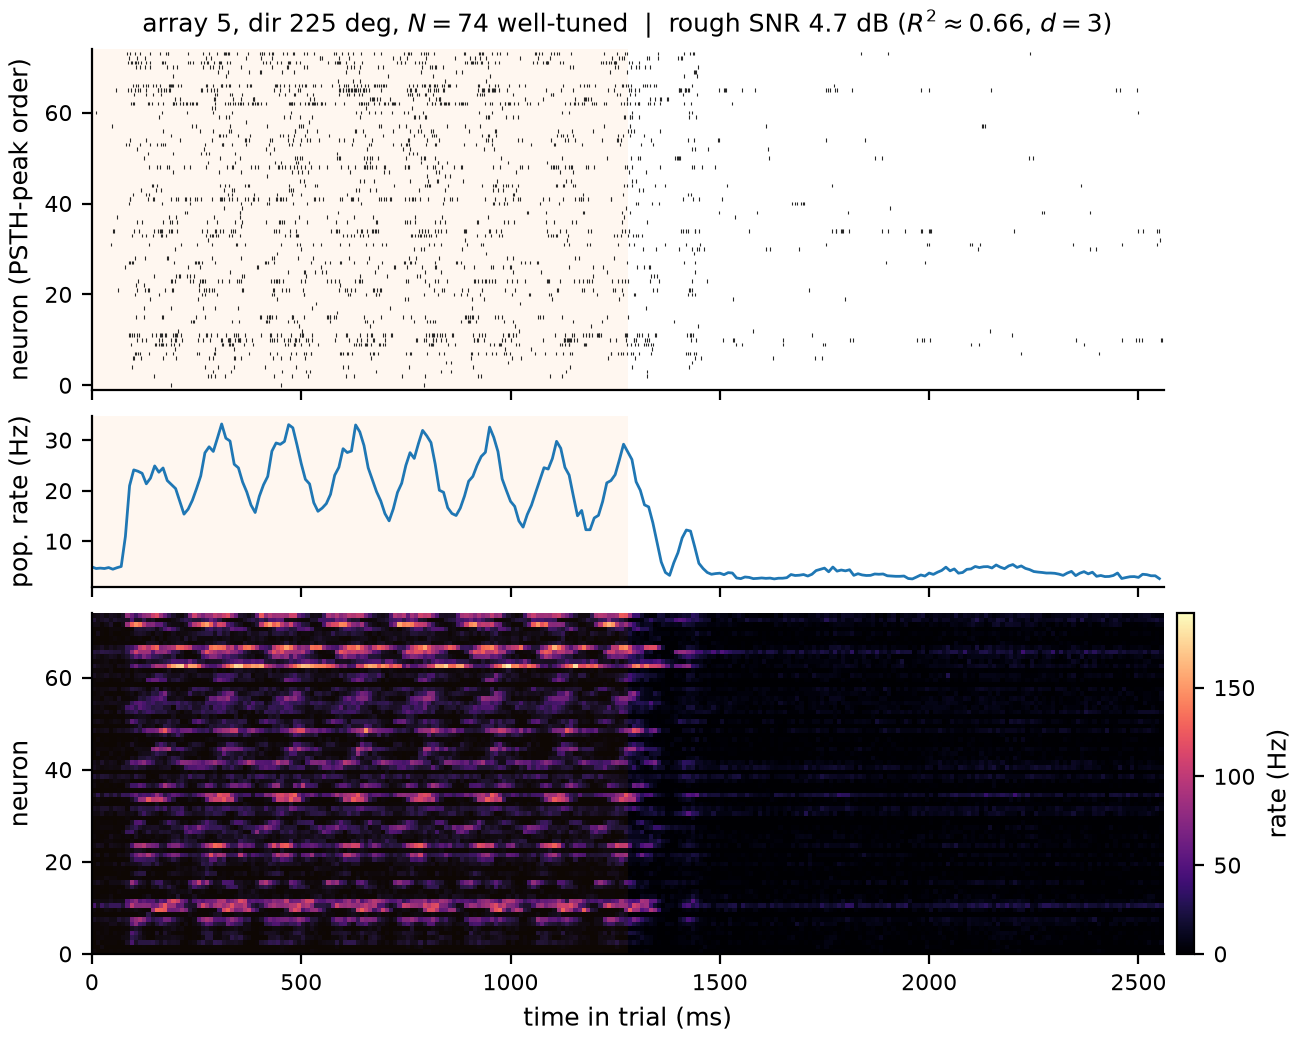
\includegraphics[width=\textwidth]{data_overview.png}
  \caption{Graf array 5, direction \ang{225} ($N{=}74$ well-tuned units), over one trial
    (stimulus window shaded). \textbf{Top:} single-trial raster (neurons ordered by PSTH
    peak time). \textbf{Middle:} trial-averaged population rate -- the \SI{6.25}{Hz} grating
    drive during the stimulus, decaying after offset. \textbf{Bottom:} per-neuron
    trial-averaged PSTH. Fisher-information SNR bound $\approx\!\SI{4.7}{dB}$ at $d{=}3$.}
  \label{fig:data}
\end{figure}

\begin{figure}[t]
  \centering
  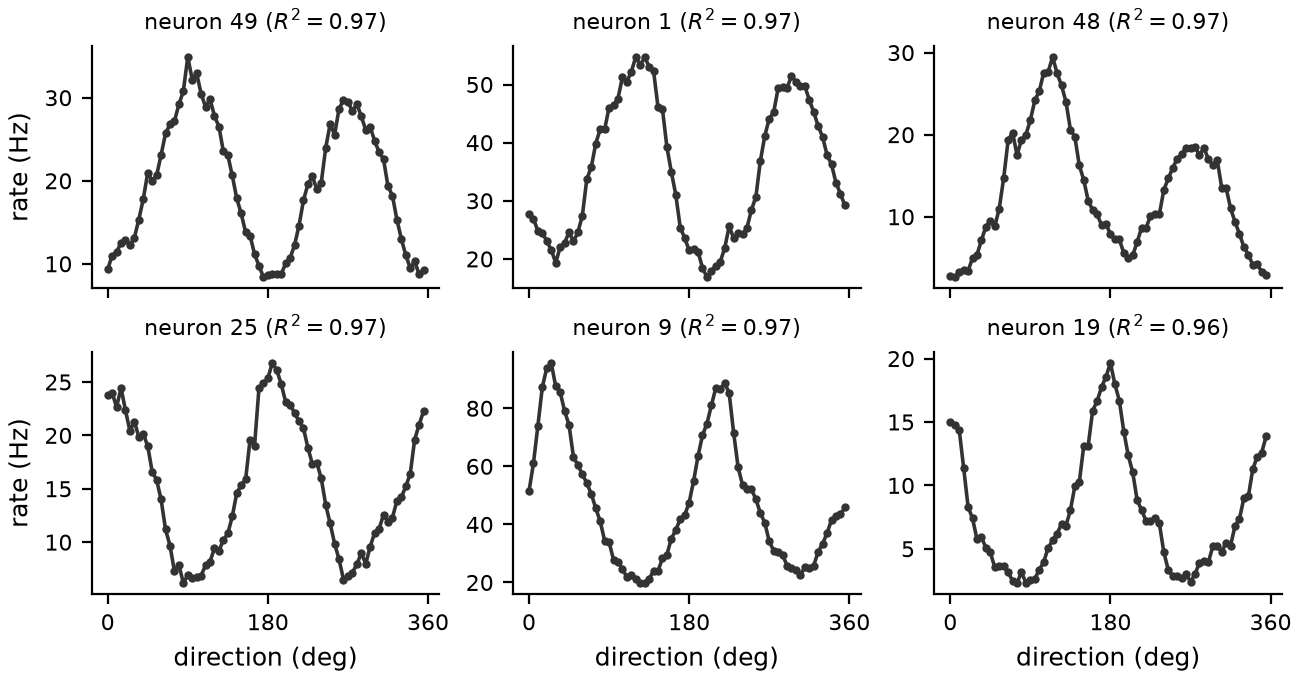
\includegraphics[width=\textwidth]{tuning_curves.png}
  \caption{Orientation tuning for the six best-fit well-tuned neurons (gray: mean
    stimulus-window rate vs direction; red: the sum-of-two-von-Mises fit). The per-panel
    $R^2$ is the \emph{tuning-fit} $R^2$ that defines the well-tuned criterion
    ($R^2\!\ge\!0.75$), distinct from the predictive log-likelihood (PLL,
    \cref{sec:criterion}) or the forecast accuracy reported later.}
  \label{fig:tuning}
\end{figure}

\begin{figure}[t]
  \centering
  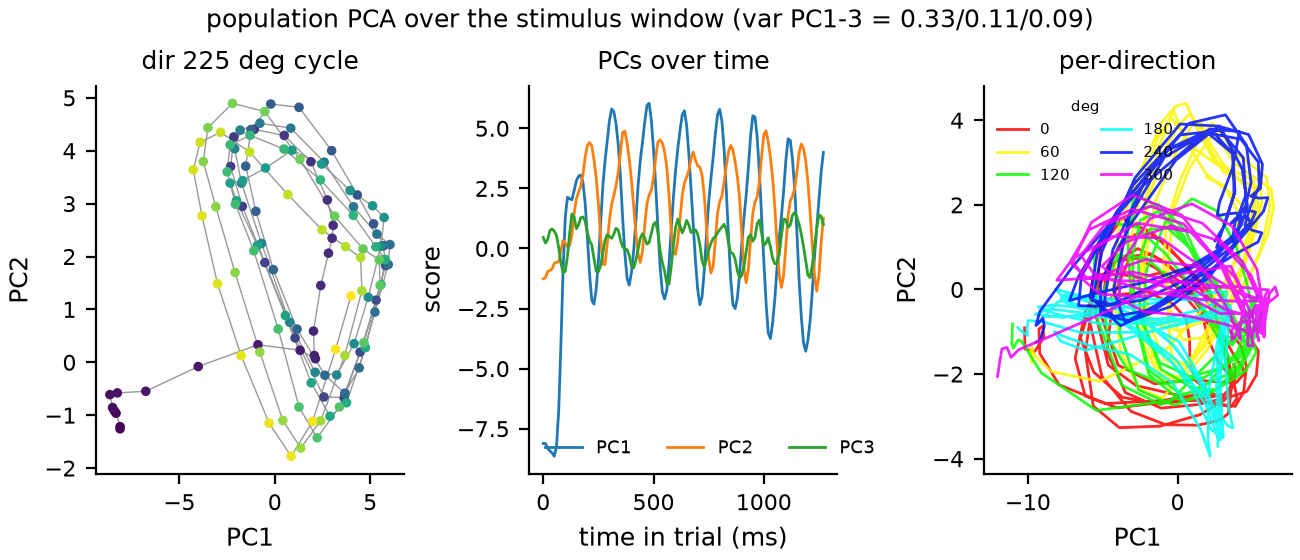
\includegraphics[width=\textwidth]{pca_traj.png}
  \caption{PCA of the population log-rate feature over the stimulus window (fit on the
    per-direction trial averages). \textbf{Left:} the PC1--PC2 trajectory for the strongest
    direction (colored by time) -- a noisy limit cycle. \textbf{Middle:} the three PC scores
    over time, oscillating at the grating frequency. \textbf{Right:} per-direction
    trajectories (circular color scheme): distinct loops carry the orientation information.}
  \label{fig:pca}
\end{figure}

\section{Method}
\paragraph{Forward step and objective.}
Each bin maximizes one filtering-step ELBO,
\begin{equation}
  \mathcal{L}(\theta) = \underbrace{\E_{q(x_t)}\!\log p(y_t\mid x_t)}_{\text{reconstruction}}
  + \underbrace{\E_{q(x_t)}\!\log p\big(x_t \mid \tilde x_{t-1},\theta\big)}_{\text{dynamics}}
  + \underbrace{H\big(q(x_t)\big)}_{\text{entropy}},
  \label{eq:elbo}
\end{equation}
where $q_t=\mathcal N(\mu_t,\Sigma_t)$ is the recognition posterior, $\tilde x_t$ a
reparameterized sample, $p(y_t\mid x_t)$ a Poisson likelihood with per-bin rate
$\lambda_t=\exp(Cx_t+b)$, and the dynamics term is Gaussian about the RBF velocity flow
$x_t=\tilde x_{t-1}+f(\tilde x_{t-1})$. Parameters are learned by a hybrid per-step scheme: a
stochastic-gradient (Adam) ascent step on \cref{eq:elbo} (training the recognition network
and the flow weights) plus closed-form non-gradient updates of the likelihood noise. The
latent is reset to the prior at each trial onset (per-trial reset).

\paragraph{Unknown readout: scale-fixed CCIPCA and the projection encoder.}
The \emph{readout} is the loading $(C,b)$ of the Poisson decoder $\lambda_t=\exp(Cx_t+b)$; it
is unknown and estimated online by CCIPCA on a causal, link-matched feature
$\tilde g(y)=\log(\nu_t+\epsilon)$, where $\nu_t$ is a leaky integrator of the counts,
$\epsilon$ a small offset, and the running mean of $\tilde g$ is $b$. CCIPCA maintains $m$
($=$ the latent dimension) vectors $\{v_i\}$ converging to $\lambda^{\mathrm g}_i e_i$ (eigenvalue $\times$ eigenvector
of $\Sigma_g=\E[(\tilde g-b)(\tilde g-b)^\trp]=U\Lambda U^\trp$); the $i$-th column of $C$ is
$\hat v_i\sqrt{\norm{v_i}}=e_i\sqrt{\lambda^{\mathrm g}_i}$ (with $\hat v_i=v_i/\norm{v_i}$),
which whitens the recognition input,
$\cov(\Renc)=\Lambda^{-1/2}U^\trp\Sigma_g U\Lambda^{-1/2}=\identity$. For this whitening to
hold online the warm start must seed $\{v_i\}$ at the same \emph{covariance} scale
($\norm{v_i}=\lambda^{\mathrm g}_i$) the streaming update converges to; seeding from the
\emph{scatter} ($\norm{v_i}\approx T\lambda^{\mathrm g}_i$ over a warm-up window of $T$
samples) makes the loading shrink by $\sim\!\sqrt T$ over training and the latent inflate.
Seeding from the feature covariance (scatter divided by the sample count) pins the loading
and $\cov(\Renc)$ across training (\cref{fig:scalefix}); this is the condition under which
the V1 latent does not inflate. The recognition reads the projection
$\Renc=C^{+}(\tilde g(y)-b)$; $(C,b)$ is Procrustes-anchored into the decoder every $K$ steps
(the refresh interval).

\paragraph{Growing RBF flow and a curvature regularizer.}
\label{sec:curv}
The velocity is $f(x)=\sum_j \phi_j(x)\,W_{j,:}$ with Gaussian RBFs
$\phi_j(x)=\exp(-\norm{x-c_j}^2/2w_j^2)$ (centers $c_j$, widths $w_j$, weights $W$); the basis
is seeded by $k$-means on the warm-up latent buffer and grown by novelty (a new center, with a
resource-allocating weight init, where the maximum basis activation falls below a threshold
$\theta_{\mathrm{grow}}$). Trained by gradient alone with a large basis, the one-step map fits
per-bin spike noise into a jagged velocity field. We add a closed-form penalty on the field
\emph{curvature}, which suppresses high-frequency wiggle while leaving an affine/rotational
field (a limit cycle) unpenalized. With $\partial^2\phi_j/\partial x\partial x^\trp=
\phi_j\big[(x-c_j)(x-c_j)^\trp/w_j^4 - I/w_j^2\big]$,
\begin{equation}
  H_a(x)=\frac{\partial^2 f_a}{\partial x\,\partial x^\trp}
        =\sum_j W_{j,a}\,\phi_j(x)\Big[\tfrac{(x-c_j)(x-c_j)^\trp}{w_j^4}-\tfrac{I}{w_j^2}\Big],
  \qquad
  R_2(x)=\sum_a \norm{H_a(x)}_F^2 .
  \label{eq:curv}
\end{equation}
The gradient step ascends the \emph{penalized} objective $\mathcal{L}-\lambda\,\E_t R_2(x_t)$,
evaluated at the filtered mean each step; the weight $\lambda$ (distinct from the Poisson rate
$\lambda_t$ and the CCIPCA eigenvalues $\lambda^{\mathrm g}_i$) controls smoothness, $\lambda{=}0$
recovers the original ELBO, and the reconstruction, recognition, and closed-form updates are
untouched. Smoothing the field changes the trajectory's roughness but, as we show, not its
forecast accuracy.

\paragraph{Multi-step rollout training of the flow.}
The one-step ELBO trains $f$ to predict the next \emph{observation-corrected} state, which does
not directly constrain the autonomous free-run. After the online pass we therefore fine-tune the
flow weights $W$ on a multi-step rollout: from each start $t$ in the steady-state window (bin
$\ge t_0$, past the onset transient) we free-run the flow with no observations,
$\hat x^{0}=\mu_t$, $\hat x^{j}=\hat x^{j-1}+f(\hat x^{j-1})$, and match a target trajectory,
\begin{equation}
  \mathcal{L}_{\text{roll}} = \frac{1}{k}\sum_{t}\sum_{j=1}^{k}\big\lVert \hat x^{j}-\mu_{t+j}\big\rVert^2,
  \label{eq:roll}
\end{equation}
descended with respect to $W$ only (detached targets; frozen centers, widths, decoder, and
readout; gradient clipped through the $k$-step recurrence). This is non-causal training on a
buffered trajectory; inference stays causal and per-bin. We vary three controls: the
\emph{target} $\mu$ -- the single-trial filtered means, the stimulus-locked trial-average orbit,
or that orbit folded into one period and tiled (an exactly-periodic target); the \emph{horizon}
$k$, swept on a curriculum that unlocks longer free-runs in blocks and mixes the unlocked lengths
(from half a cycle up to ten cycles); and the gradient-clip norm. The horizon matters because a
slow per-cycle amplitude drift is invisible to a short rollout ($<\!3\%$ over three cycles) and
only becomes a sizable penalty over many cycles.

\paragraph{Characterizing the autonomous attractor.}
To probe the free-run dynamics independent of any forecast, we free-run the learned flow for
\num{400} cycles from a dense range of initial amplitudes along the cycle's radial direction and
record the per-cycle peak radius in the leading decoded-variance plane (\cref{eq:rot}) -- the
\emph{amplitude return map}. An attracting limit cycle draws these initial radii onto one nonzero
ring (attraction from inside and outside); a point attractor draws them all to zero. As a local
companion diagnostic we take the eigenvalues of the flow-map Jacobian $\partial F/\partial x$,
$F(x){=}x{+}f(x)$, by finite differences at the tail mean of the free-run, and write
$\rho{=}\max_i\abs{\lambda_i}$; near a true cycle's enclosed fixed point $\rho{>}1$ (unstable
spiral) and near a stable focus $\rho{<}1$. This is a Jacobian \emph{at the orbit centroid}, not
at a solved fixed point (the centroid need not satisfy $f{=}0$), so we read it only as a
near-marginal indicator, not a stability proof -- and indeed $\rho$ straddles $1$ across fits.

\paragraph{Train/validation/test split and replay training.}
The stream opens with a coverage warm-up (dynamics off) over which the readout is fit and the
latent means buffered; the RBF flow is then initialized once and turned on. The 30 train
trials are replayed for $E$ epochs in a randomized order, with the posterior reset at each
trial onset, so the readout and flow keep adapting while no information leaks across trials.
Each epoch is one strictly causal per-bin pass (no minibatching). Evaluation freezes the model
and runs the held-out trials.

\begin{algorithm}[t]
\caption{\svjf{} on V1: warm-up then $E$ replay epochs (per-trial reset). Key additions -- the
  scale-fixed CCIPCA warm-start, the curvature penalty, and the growing basis -- are boxed.}
\label{alg:svjf}
\begin{algorithmic}[1]
\Require trials; warm-up trials; refresh interval $K$; curvature weight $\lambda$
\State init readout state $\nu,b,\{v_i\}$; posterior $q\gets\varnothing$; feature buffer
  $\mathcal G\gets[\,]$, latent buffer $\mathcal X\gets[\,]$
\Statex \textit{Warm-up (warm-up trials, dynamics off): fit the readout, buffer the feature and the latent means}
\For{each bin $y_t$ in the warm-up trials}
  \State update $\nu,b$; CCIPCA step on $\tilde g(y_t)-b$; filter $y_t$ (dynamics off);
    append $\tilde g(y_t)-b$ to $\mathcal G$ and $\mu_t$ to $\mathcal X$
\EndFor
\State \fbox{$v_i\gets \lambda^{\mathrm g}_i e_i$ from the \emph{covariance} (not scatter) of $\mathcal G$}\Comment{scale fix}
\State seed RBF centers by $k$-means on the latent buffer $\mathcal X$; turn the dynamics on
\Statex \textit{Online ($E$ randomized replay epochs over the train trials; reset $q$ each trial onset)}
\For{each bin $y_t$}
  \State $\mu_t,q\gets\textsc{VjfFilter}(y_t,\,C^{+}(\tilde g(y_t)-b),\,q)$ \Comment{recognition + flow}
  \State \fbox{gradient step on $\mathcal L-\lambda\,R_2(\mu_t)$}\Comment{curvature penalty, \cref{eq:curv}}
  \State \fbox{\textbf{if} novelty$(\tilde x_t)<\theta_{\mathrm{grow}}$: add an RBF center (resource-allocating init)}\Comment{growing basis}
  \If{$t\bmod K=0$} Procrustes-refresh $(C,b)$ into the decoder \EndIf
\EndFor
\end{algorithmic}
\end{algorithm}

\paragraph{The forecast-reconstruction criterion.}
\label{sec:criterion}
The model-selection metric is \emph{future forecasted reconstruction}. From start phases
$t_0$ in the steady-state window (from bin \num{32}, the end of the second cycle, past the onset
transient), we free-run the flow with no observations after $t_0$, decode it to a predicted
per-bin rate, and score that forecast against the future spike counts by the Poisson deviance
\begin{equation}
  D(k)=2\textstyle\sum\big[\,n\log(n/\lambda)-(n-\lambda)\,\big],
  \label{eq:dev}
\end{equation}
where $\lambda$ is the forecast's expected count per \SI{10}{ms} bin, $n$ the observed count,
$n\log(n/\lambda)\!:=\!0$ at $n{=}0$, and the sum runs over neurons, the $k$ forecast bins, the
start phases, and the held-out trials. We report the \emph{forecast accuracy}
$a_k=1-D_{\mathrm{model}}(k)/D_{\mathrm{base}}(k)$ relative to two baselines: \emph{persistence}
(hold the model's $t_0$ rate) and the stimulus-locked \emph{PSTH} (the train trial-average at
each absolute bin); $a_k{=}1$ is an exact forecast, $0$ ties the baseline, $a_k{<}0$ is worse.
The pre-declared selection score is $S=0.5\,a_8+0.3\,a_{16}+0.2\,a_{32}$ versus persistence,
gated by a filtered PLL within a margin of the PSTH ceiling; we additionally report $a_k$ out to
$k{=}96$ (six cycles, the longest the trials admit). For the across-horizon comparison
(\cref{fig:horizon}, \cref{tab:rollout}) the start set is held fixed at the launch phases that
admit the longest horizon, so every $a_k$ is scored on a common set of starts (and $S$ there is on
this common subset, not the full selection grid). Scoring the decoded rate against the
observed future spikes -- not a latent-space $R^2$ -- removes the affine-overfit loophole of
self-referential latent metrics. We also report the filtered \emph{leave-one-neuron} PLL
(bits/spike; \cite{vlgp}): for each held-out neuron, filter the trial from the other neurons'
projection and score its predicted rate against the counts, relative to a homogeneous-Poisson
baseline (0 = mean-rate). The \emph{PSTH ceiling} is the same PLL with the stimulus-locked
trial-averaged rate as predictor.

\paragraph{Ordering the latent factors for display.}
The VJF latent is identifiable only up to an invertible linear transform: $(x_t,C)\mapsto(Mx_t,
CM^{-1})$ leaves the decoded log-rate $\eta_t=Cx_t+b$ unchanged, so the individual factor axes
are not unique. We order the factors by the variance they explain in the \emph{decoded
log-rate} -- the neural-data signal, whose scale (unlike the latent's) is fixed by the readout.
Let $\tilde X$ be the centered latent path over a trial (rows $(x_t-\bar x)^\trp$,
$\bar x$ the trial-averaged latent), so the centered decoded log-rate is $\tilde H=\tilde X
C^\trp$. With its singular value decomposition $\tilde H=U\Sigma V_L^\trp$, where
$V_L=[r_1,\dots,r_L]$ are the leading $L$ right singular vectors ($\mathrm{rank}\,\tilde
H\le L$), define
\begin{equation}
  W = C^\trp V_L,\quad\text{columns } w_i=C^\trp r_i, \qquad z_t = W^\trp(x_t-\bar x),
  \label{eq:rot}
\end{equation}
so the scores are exactly the decoded-log-rate principal-component time courses,
$Z=\tilde X W = \tilde H V_L = U\Sigma$, and factor $i$ ($z_{t,i}=w_i^\trp(x_t-\bar x)$)
explains the $i$-th largest share $\Sigma_{ii}^2/\sum_j\Sigma_{jj}^2$ of the decoded-log-rate
variance ($Z^\trp Z=\Sigma^2$ on the reference path). $W$ is a decoder-induced linear
projection -- the decoded-log-rate PC-score map -- \emph{not} an orthogonal rotation
($W^\trp W\ne I$ in general). Because $C$ here has eig-normalized columns
($C=U_g\Lambda_g^{1/2}$, the scale-fixed CCIPCA loading), the latent is approximately whitened,
so $W$ is close to a reordering and rescaling of the existing factors rather than a substantive
recombination. The same $W,\bar x$ are applied to the single-trial filtered latent and the
free-run forecast (\cref{fig:freerun}).

\begin{figure}[t]
  \centering
  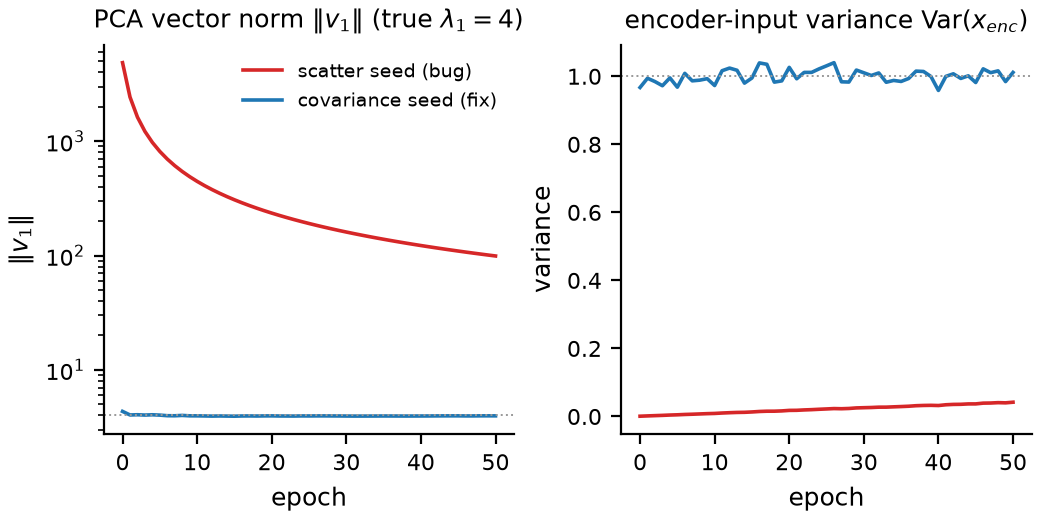
\includegraphics[width=0.8\textwidth]{scale_fix.png}
  \caption{The CCIPCA warm-start scale requirement, on stationary Gaussian data (true variances
    $\lambda^{\mathrm g}=[4,1]$). \textbf{Left:} the leading PCA-vector norm $\norm{v_1}$. The
    scatter seed (red) starts $\sim\!T$ too large and drifts down for the entire run; the
    covariance seed (blue) sits at the true $\lambda^{\mathrm g}_1$. \textbf{Right:} the
    encoder-input variance $\cov(\Renc)$ is pinned at $1$ by the covariance seed (blue) but
    migrates under the scatter seed (red). A drifting loading is what inflates the \svjf{}
    latent, so the covariance-scale seed is required.}
  \label{fig:scalefix}
\end{figure}

\section{Results}
\paragraph{Reconstruction reaches the PSTH ceiling.}
With observations, \svjf{} reconstructs held-out neurons as well as trial-averaging: the
filtered leave-one-neuron PLL on the test trials is \SI{0.69}{} bits/spike (mean over fits), at
or slightly above the stimulus-locked PSTH ceiling (\num{0.64}). Reconstruction is therefore not
the bottleneck, and every searched configuration clears the reconstruction gate. The question is
what the \emph{autonomous dynamics} are, and whether they forecast.

\paragraph{The autonomous free-run sustains an oscillation, not a collapse to the mean.}
A single free-run reads as ``decaying'': launched from the filtered state at $t_0$, its leading
factors lose amplitude over the trial (\cref{fig:freerun}). That reading is incomplete.
Free-running the learned flow from a dense range of initial amplitudes, the trajectories settle
toward a \emph{nonzero} ring rather than the origin (\cref{fig:limitcycle}, return maps;
\cref{fig:phaseportrait}) -- the apparent ``decay'' is the high-amplitude filtered start (whose
single-trial amplitude exceeds the trial-average orbit) relaxing inward toward that ring. The
free-run sustains the oscillation for many cycles; it does not collapse to the mean. Whether the
ring is a true attracting limit cycle or a very slowly decaying focus is, however,
\emph{near-marginal}: the flow map's eigenvalues at the cycle center lie near the unit circle and
straddle it across fits (\cref{fig:limitcycle}, lower panels; \cref{tab:rollout}, $\rho$), and the
ring amplitude is weakly identified from $\sim$8-cycle trials (ring/data $\approx\!0.2$--$1.1$
across fits and strategies). The qualitative conclusion is robust -- the dynamics sustain an
oscillation rather than collapsing -- but the formal stability and the amplitude are not pinned
down by these short trials.

\begin{figure}[t]
  \centering
  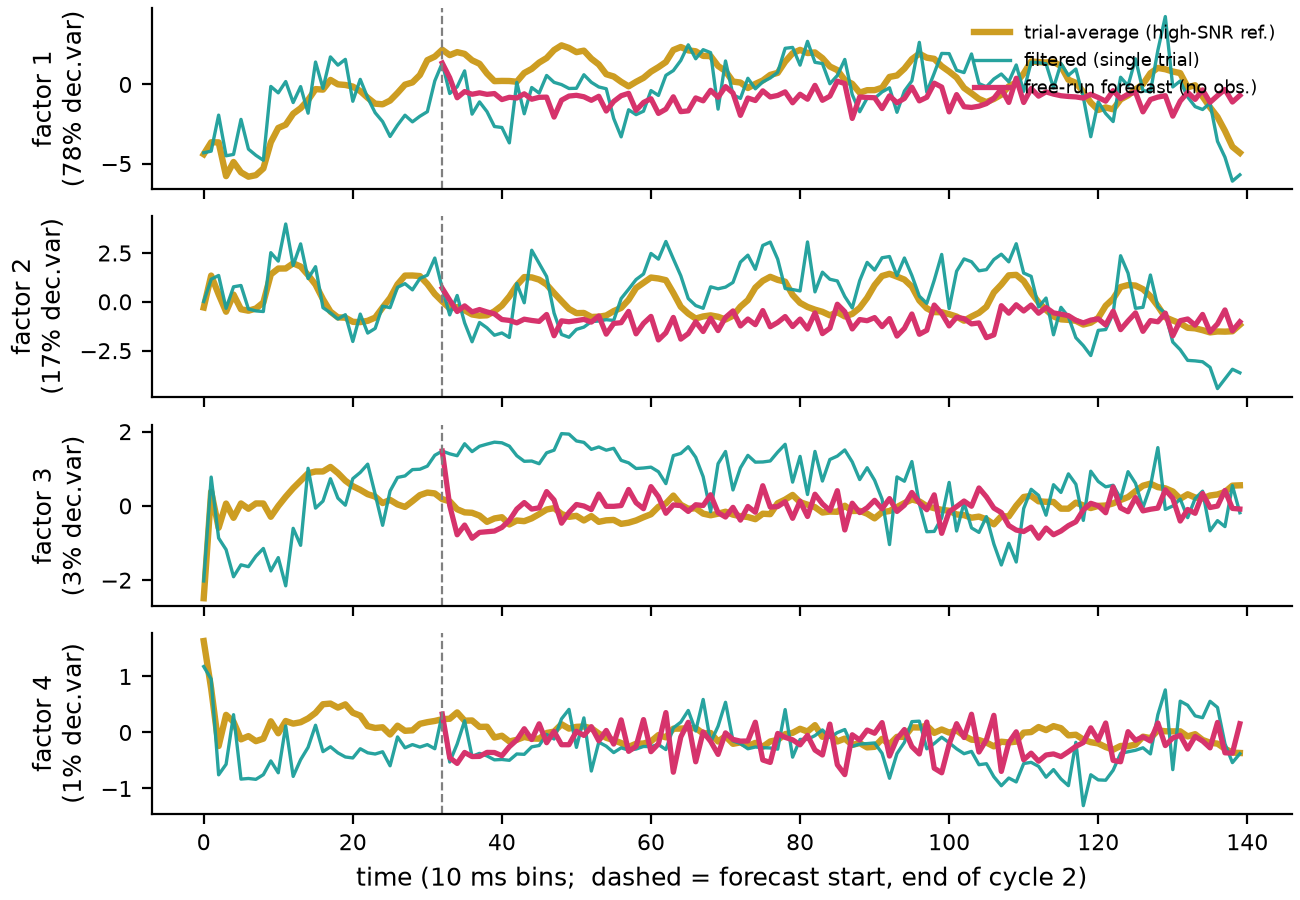
\includegraphics[width=\textwidth]{forecast_time.png}
  \caption{Held-out free-run of the learned flow over one test trial, each VJF factor ordered by
    the decoded-log-rate variance it explains (\cref{eq:rot}; \% in each panel). \textbf{Gold:}
    the trial-averaged latent (the high-SNR reference cycle). \textbf{Teal:} the single-trial
    filtered latent (with spikes). \textbf{Crimson:} the autonomous free-run launched at the end
    of the second cycle (dashed line; past the onset transient), with \emph{no} observations
    after $t_0$. Over the trial the free-run loses amplitude -- but this is the high-amplitude
    single-trial start relaxing onto the sustained oscillation, not a collapse to the mean
    (\cref{fig:limitcycle}).}
  \label{fig:freerun}
\end{figure}

\begin{figure}[t]
  \centering
  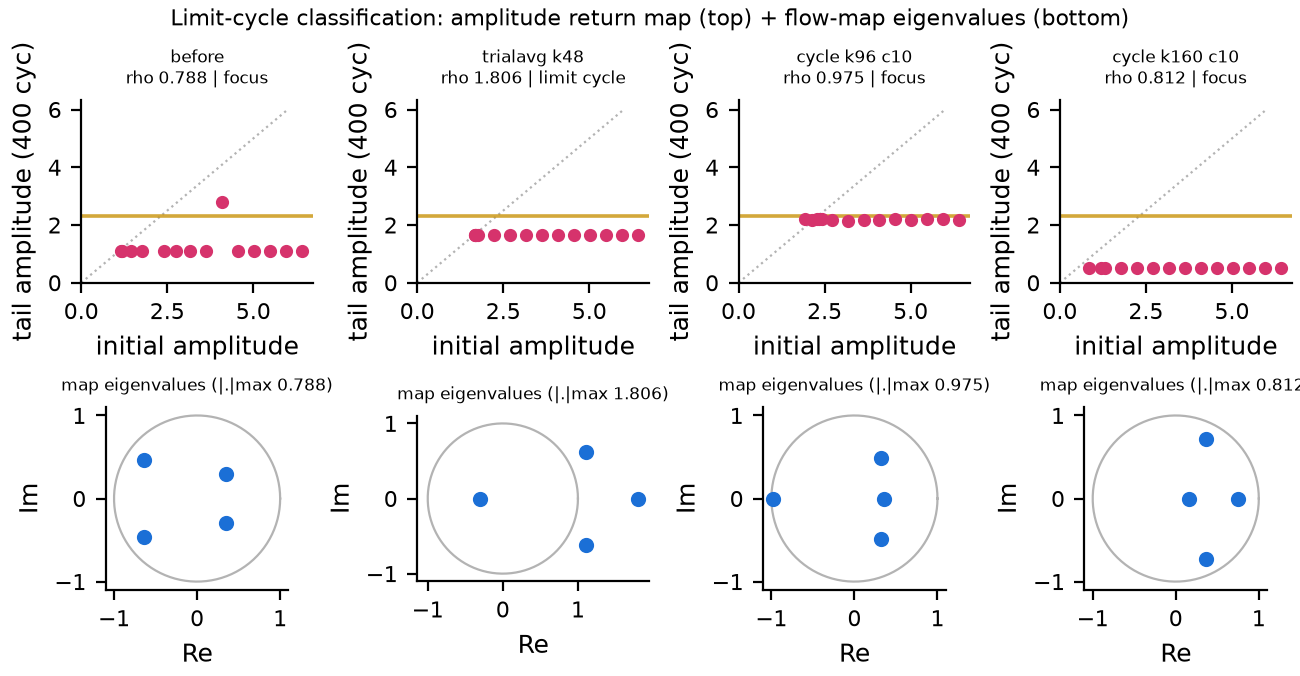
\includegraphics[width=\textwidth]{limit_cycle_class.png}
  \caption{\textbf{Near-marginal autonomous dynamics: a sustained oscillation of weakly-identified
    stability.} One representative fit per strategy. \textbf{Top -- amplitude return map:}
    free-running the flow for \num{400} cycles from a dense range of initial amplitudes, the tail
    amplitude (leading decoded-variance plane) settles toward a nonzero ring (gold line:
    data-orbit amplitude), \emph{not} zero -- the free-run sustains an oscillation. The ring
    amplitude varies across strategies and fits (\cref{tab:rollout}). \textbf{Bottom -- flow-map
    eigenvalues:} the largest eigenvalue lies \emph{near the unit circle} and crosses it from fit
    to fit (here $0.79$/$1.81$/$0.98$/$0.81$), so whether the ring is a true attracting limit
    cycle (a pair outside the circle) or a slowly decaying focus (inside) is not reliably
    identified from these short trials.}
  \label{fig:limitcycle}
\end{figure}

\begin{figure}[t]
  \centering
  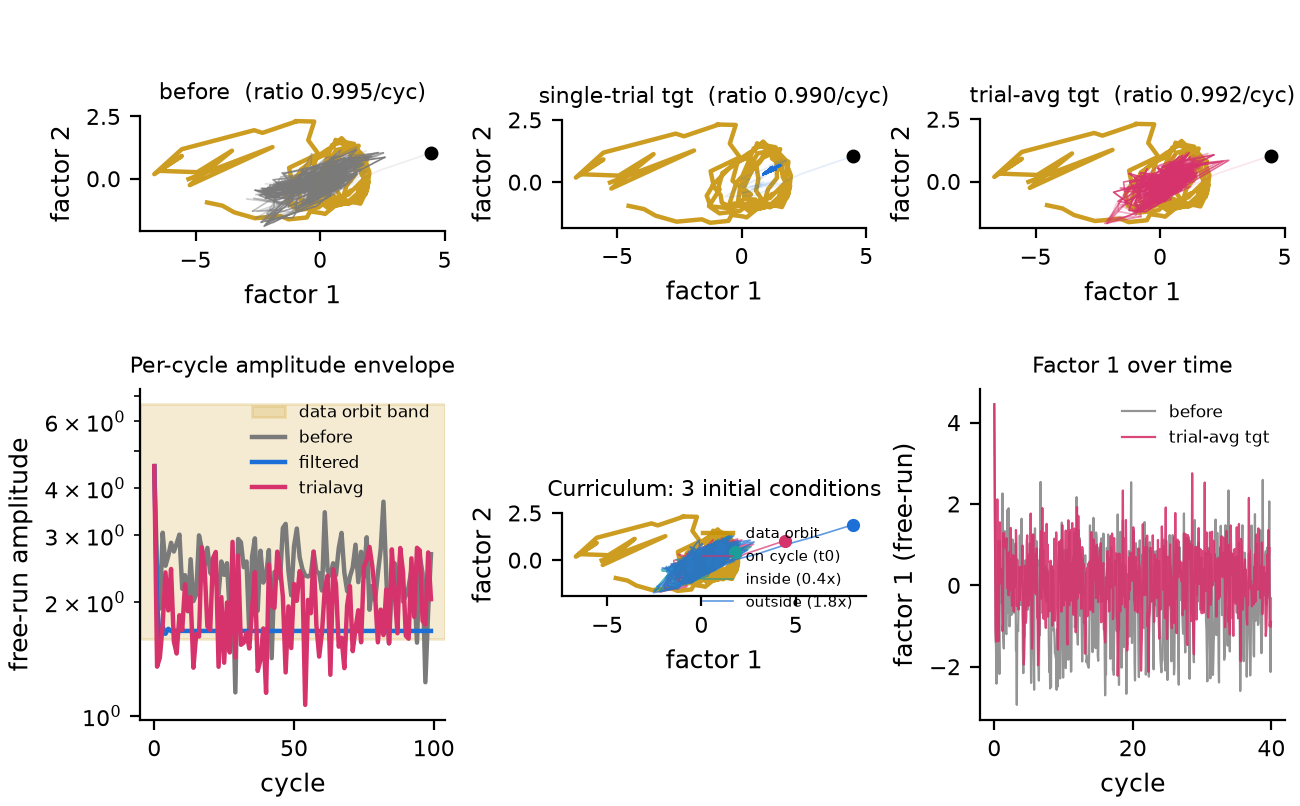
\includegraphics[width=\textwidth]{rollout_diag.png}
  \caption{The free-run in the leading decoded-variance plane (one fit; one-step and two rollout
    targets). \textbf{Top:} phase portraits -- the autonomous free-run (colored, fading over
    \num{40} cycles) launched from the high-amplitude $t_0$ state spirals \emph{inward} toward the
    data orbit (gold), per-cycle amplitude ratios near $1$ (titles). \textbf{Bottom left:} the
    per-cycle amplitude envelope over \num{100} cycles settles toward a finite ring, not zero.
    \textbf{Bottom middle:} three initial conditions (inside / on / outside) under one flow.
    \textbf{Bottom right:} factor-1 free-run over time. The apparent ``decay'' of a single trace
    is relaxation onto the ring; the ring itself is the attractor of \cref{fig:limitcycle}.}
  \label{fig:phaseportrait}
\end{figure}

\paragraph{No autonomous free-run consistently beats the phase-locked PSTH; forecasting rewards shrinkage.}
Scored against the held-out future spikes from half a cycle to six (\cref{fig:horizon}), no flow
\emph{consistently} beats the stimulus-locked PSTH: the most contractive flow reaches parity near
one cycle ($a_{16}$ marginally positive for two of three seeds), but every flow falls increasingly
below the PSTH as the horizon grows. This is expected and not a model failure: the PSTH ``knows''
the absolute phase at every future bin, whereas an autonomous free-run propagates the phase from
$t_0$ and accumulates phase error. Against persistence the picture is a trade-off
(\cref{tab:rollout}). On the short-horizon selection score $S$, the only configuration that
consistently beats persistence is the most \emph{contractive} one -- the single-trial rollout
($S{=}{+}0.015\!\pm\!0.002$), whose flow hugs the trial-average orbit and shrinks single-trial
variance -- and it is also the least-bad against the PSTH ($a_8{\approx}{-}0.001$). Every
configuration that \emph{enlarges or sustains} the oscillation (the one-step flow, and the
periodic/long-horizon rollouts) scores \emph{worse} on $S$. The ranking is preserved across
horizons, though at the longest horizons persistence is itself so weak that most flows approach or
edge above it (\cref{fig:horizon}, left). Under single-trial noise and free-run phase drift, the
minimum-deviance predictor regresses toward the mean -- so forecast accuracy is opposed to
sustaining the oscillation.

\begin{figure}[t]
  \centering
  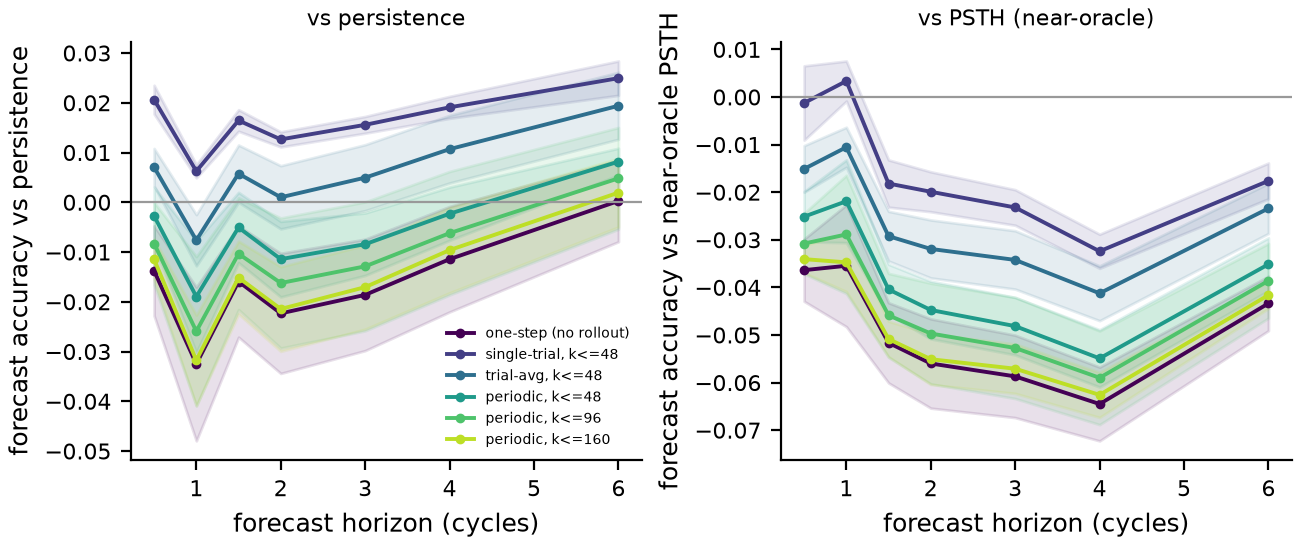
\includegraphics[width=\textwidth]{forecast_vs_horizon.png}
  \caption{Held-out forecast accuracy vs horizon (mean$\pm$s.d.\ over 3 seeds), from half a cycle
    to six. \textbf{Left, vs persistence:} the most contractive flow (single-trial rollout) leads
    at every horizon; the one-step flow and the periodic/long-horizon rollouts -- those that
    sustain the oscillation -- trail it, dipping below persistence at short horizons and rising
    toward it as persistence weakens at long horizons. \textbf{Right, vs the near-oracle PSTH:} no
    flow consistently exceeds the PSTH -- the single-trial flow only reaches parity near one cycle,
    and the gap to the PSTH widens with horizon, because the phase-locked PSTH knows the absolute
    phase a free-run must propagate.}
  \label{fig:horizon}
\end{figure}

\paragraph{A systematic rollout study: two orthogonal axes.}
We fine-tune the one-step flow with the rollout objective (\cref{eq:roll}) and scan its target,
horizon ladder, and gradient clip over three fit seeds (\cref{tab:rollout}). Two axes separate.
\emph{Forecasting:} only the short-horizon single-trial target beats persistence; the
trial-average target ties it, and the periodic targets -- which sustain the cycle most strongly
-- forecast worse as the horizon grows. \emph{Dynamics:} the rollout reshapes the attractor, but
its amplitude and stability are weakly identified from $\sim$8-cycle trials. The long-horizon
periodic target, which most directly penalizes amplitude decay, tends to enlarge the ring toward
the data orbit, but unreliably -- ring/data is $0.72\!\pm\!0.39$ across seeds (range
$0.18$--$1.18$), and the center spectral radius $\rho$ straddles $1$ -- and at a forecast cost.
Capacity is not the lever either: in the validation search the best forecast accuracy is flat
across latent dimension $L{=}3$--$5$ and \emph{drops} at $L{=}6$, with no gain past $E{=}100$
training epochs (\cref{tab:capacity}). The two goals -- a sustained oscillation and a good
single-trial forecast -- pull in opposite directions, and the rollout trades between them.

\begin{table}[t]
  \centering
  \caption{Multi-step rollout study (dir \ang{225}, $L{=}4$, \num{1600} RBF; held-out test,
    mean$\pm$s.d.\ over 3 fit seeds). Forecasting and sustained oscillation are opposed: the only
    consistent persistence-beater ($S{>}0$, \textbf{bold}) is the most contractive flow
    (single-trial target), while the flows that enlarge/sustain the oscillation (one-step,
    periodic, long horizon) forecast worse; none beats the phase-locked PSTH ($a_k$ vs PSTH
    ${<}0$) at any horizon. Ring amplitude (relative to the data orbit) and the center spectral
    radius $\rho$ (a true limit cycle would have $\rho{>}1$) are weakly identified and
    near-marginal across seeds -- $\rho$ straddles $1$ (per-seed range $\approx\!0.7$--$2.4$).
    $S$ and ring/data are mean$\pm$s.d.; $a_8$, $a_{96}$, and $\rho$ are seed means. $k_{\max}$ in
    bins (16/cycle).}
  \label{tab:rollout}
  \begin{tabular}{lccrrrcc}
    \toprule
    rollout target & $k_{\max}$ & clip & $S$ vs persist & $a_8$ PSTH & $a_{96}$ PSTH & ring/data & $\rho$ \\
    \midrule
    none (one-step)  & --  & --  & $-0.021{\scriptstyle\pm.012}$           & $-0.036$ & $-0.043$ & $0.74{\scriptstyle\pm.29}$ & $1.6$ \\
    single-trial     & 48  & 1   & $\mathbf{+0.015{\scriptstyle\pm.002}}$  & $-0.001$ & $-0.018$ & $0.52{\scriptstyle\pm.12}$ & $1.0$ \\
    trial-average    & 48  & 1   & $+0.001{\scriptstyle\pm.005}$           & $-0.015$ & $-0.023$ & $0.59{\scriptstyle\pm.08}$ & $1.7$ \\
    periodic         & 48  & 1   & $-0.009{\scriptstyle\pm.008}$           & $-0.025$ & $-0.035$ & $0.52{\scriptstyle\pm.13}$ & $1.1$ \\
    periodic         & 96  & 10  & $-0.015{\scriptstyle\pm.011}$           & $-0.031$ & $-0.039$ & $0.72{\scriptstyle\pm.38}$ & $1.5$ \\
    periodic         & 160 & 10  & $-0.020{\scriptstyle\pm.006}$           & $-0.034$ & $-0.042$ & $0.72{\scriptstyle\pm.39}$ & $1.4$ \\
    \bottomrule
  \end{tabular}
\end{table}

\begin{table}[t]
  \centering
  \caption{Capacity is not the lever. Best validation forecast accuracy $S$ vs persistence in the
    single-direction search, by latent dimension $L$: small and flat across $L{=}3$--$5$, then
    \emph{lower} at $L{=}6$. By training length the best $S$ is $+0.024/+0.018/+0.036/+0.033$ at
    $E{=}20/50/100/200$ -- no gain past $E{=}100$.}
  \label{tab:capacity}
  \begin{tabular}{lcccc}
    \toprule
    latent dimension $L$ & 3 & 4 & 5 & 6 \\
    \midrule
    best $S$ (validation)   & $+0.027$ & $+0.033$ & $+0.036$ & $+0.008$ \\
    best basis size         & 800 & 2400 & 2400 & 1600 \\
    \bottomrule
  \end{tabular}
\end{table}

\paragraph{Real-time.}
The per-bin cost of the online learning step is \SI{0.3}{ms} (frozen inference \SI{0.1}{ms}),
measured on an M-series CPU at \num{1600} RBF centers -- about \num{30}$\times$ faster than the
\SI{10}{ms} bin budget, so the basis size is not a real-time constraint. The per-timestep loop
is CPU-bound; a GPU does not help.

\section{Discussion}
On a single grating direction, \svjf{} reconstructs held-out V1 neurons online -- with an
unknown readout -- at the stimulus-locked PSTH ceiling. Beyond reconstruction, two findings
stand on orthogonal axes. The learned autonomous flow \emph{sustains an oscillation}: a dense
range of initial conditions settles toward a nonzero ring, so the free-run does not collapse to
the mean -- what looks like decay in a single trace is the high-amplitude filtered start relaxing
onto that ring. Whether the ring is a true attracting limit cycle or a slowly decaying focus is
near-marginal -- the flow-map eigenvalues lie near the unit circle and the classification varies
across fits -- and the amplitude is weakly identified from $\sim$8-cycle trials. And yet, robustly,
\emph{single-trial forecast accuracy does not reward sustaining the oscillation}. No autonomous
free-run beats the phase-locked PSTH at any horizon -- the PSTH carries absolute-phase information
a free-run must propagate and lose -- and against persistence the best forecaster is the most
contractive flow, because under single-trial noise and phase drift the minimum-deviance prediction
regresses toward the mean orbit. The multi-step rollout makes the trade-off explicit: short-horizon,
single-trial targets buy forecast accuracy by contracting; long-horizon periodic targets sustain
the oscillation but forecast worse. Beating the PSTH was never the attainable bar for an autonomous
model; the attainable bar -- dynamics that sustain the oscillation rather than collapsing to the
mean -- is met, and is best read off the dynamics directly, not off the forecast score.

\paragraph{Limitations and next steps.} The oscillation's amplitude and stability are weakly
identified from $\sim$8-cycle trials (ring/data spans $0.18$--$1.18$ across seeds and $\rho$
straddles $1$), and the cleanest periodic
target tiles the orbit beyond the observed window, assuming periodicity the data only partly
constrain; longer recordings or a phase-tolerant forecast metric (crediting correct shape under a
phase offset) would sharpen both the amplitude estimate and the forecast comparison. The
criterion -- a fully autonomous free-run scored per-bin against single trials -- is strict by
construction; giving the flow the stimulus as an input, and the multi-direction case where the
input selects the cycle, are the natural next steps.

\begin{thebibliography}{9}
\bibitem[Zhao \& Park(2020)]{zhao2020} Y.~Zhao and I.~M.~Park.
  Variational online learning of neural dynamics. \emph{Front. Comput. Neurosci.}, 2020.
\bibitem[Zhao \& Park(2017)]{vlgp} Y.~Zhao and I.~M.~Park.
  Variational latent Gaussian process for recovering single-trial dynamics from population
  spike trains. \emph{Neural Computation}, 29(5):1293--1316, 2017.
\bibitem[Graf et al.(2011)]{graf2011} A.~B.~A.~Graf, A.~Kohn, M.~Jazayeri, J.~A.~Movshon.
  Decoding the activity of neuronal populations in macaque primary visual cortex.
  \emph{Nat. Neurosci.}, 14(2):239--245, 2011.
\end{thebibliography}

\end{document}
